Este capítulo trata das etapas do desenvolvimento do Sistema Gerenciador de \textit{Workflows} Científicos para a plataforma BioNimbuZ, e as alterações necessárias para que ele fosse suportado pelo atual estado do sistema. Primeiramente, na Seção \ref{cap5sec1} é apresentado o funcionamento do BioNimbuZ antes do desenvolvimento do sistema gerenciador de \textit{workflows}, o qual era executado através de um \textit{terminal}. Os novos requisitos do sistema são apresentados na Seção \ref{cap5sec2}. Com esses requisitos, foi proposta uma nova arquitetura para o sistema, a qual é apresentada na Seção \ref{cap5sec3}. A Seção \ref{cap5sec4} mostra os detalhes de como a Aplicação \textit{Web} foi desenvolvida para dar suporte ao Sistema Gerenciador de \textit{Workflows}. Na Seção \ref{cap5sec5}, são expostos os motivos da contrução de um novo componente da arquitetura de \textit{software}, chamada Camada de Comunicação, responsável por realizar a troca de mensagens entre o Núcleo do BioNimbuZ e a Aplicação \textit{Web} utilizando \textit{webservices REST}. Por último, na Seção \ref{cap5sec6} são apresentadas as alterações feitas no BioNimbuZ para suportar esse novo modo de acesso, composto pela aplicação \textit{web} e a camada de comunicação.

\section{Do \textit{terminal} para a Interface \textit{Web}} \label{cap5sec1}

O BioNimbuZ primeiramente projetado e implementado por Hugo Saldanha [3] era acessado via \textit{terminal}. Nele, o usuário digitava uma série de comandos, os quais eram processados e executados pelo servidor do BioNimbuZ, e então recebia de volta o resultado daquele comando. Essa forma não era nem intuitiva nem amigável para o usuário, pois exigia que o mesmo conhecesse a execução de comandos através de um \textit{terminal}. Para, por exemplo, submeter uma sequência de passos, ou \textit{jobs}, formando assim um \textit{workflow}, o usuário deveria executar diversos comandos em sequência, ou seja, o usuário era quem gerenciava todos os passos de seu \textit{workflow}. Outro ponto negativo dessa abordagem era o fato de que o usuário não poderia acessar o sistema, ver os \textit{jobs} submetidos ou visualizar seus arquivos de qualquer lugar, pois era necessário realizar o \textit{download} do executável do BioNimbuZ em sua máquina local. Uma das vantagens da nova abordagem de sistema baseado em tecnologias \textit{web} é a acessibilidade provida pela \textit{Internet}. Dessa forma, o usuário pode, por exemplo, iniciar um \textit{workflow} em seu laboratório, concluí-lo e submetê-lo em casa e verificar sua execução pelo celular. 

Na abordagem anterior, baseada em \textit{terminal}, era necesário realizar o \textit{download} do \textit{.JAR} (\textit{Java Archive}) do projeto e executá-lo via linha de comando. A Figura \ref{fig:terminal_bionimbuz} mostra a interface percebida pelo usuário ao se executar o BioNimbuZ no sistema operacional Linux:

\begin{figure}[H]
	\centering
	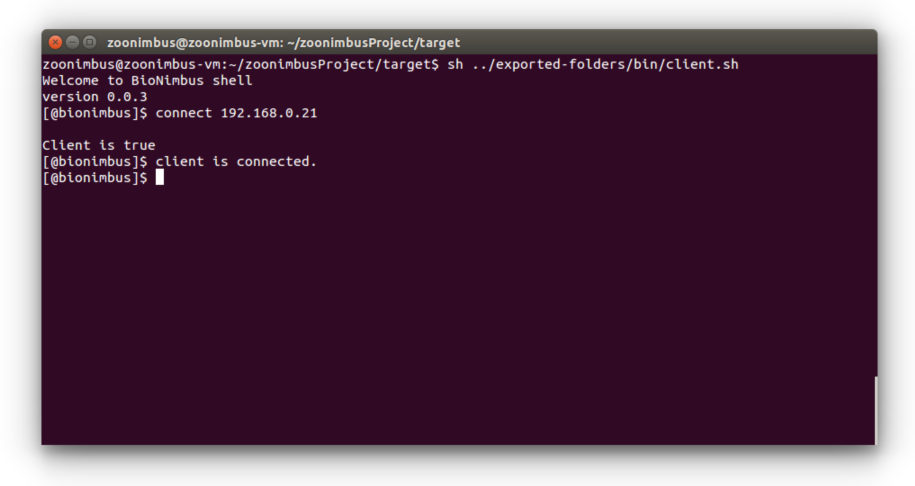
\includegraphics[scale=0.49]{terminal_bionimbuz.png}
	\caption{\textit{Terminal} do BioNimbuZ.}
	\label{fig:terminal_bionimbuz}
\end{figure}

Dessa forma, utilizando a interface mostrada na Figura \ref{fig:terminal_bionimbuz}, para o usuário submeter um \textit{workflow} com dois passos, a seguinte sequência de comandos deveria ser executada:

\begin{enumerate}
	\item [1.] Executar o comando \textbf{\textit{connect}} para se conectar ao BioNimbuZ, passando o IP da máquina servidora como argumento do comando;
    \item [2.] Enviar cada arquivo a partir do comando \textbf{\textit{upload}}, passando o caminho do arquivo à ser enviado;
    \item [3.] Com todos os arquivos enviados, submeter o comando \textbf{\textit{start}} passando o identificador do primeiro serviço (nesse caso, serviço se refere ao software computacional a ser executado naquele \textit{job} e uma lista contendo os serviços disponíveis era mostrada a partir do comando \textbf{\textit{services}}), a lista de arquivos de entrada e a lista de arquivos de saída;
    \item [4.] A partir do início de um \textit{job} era possível verificar seu \textit{status} com o comando \textbf{\textit{status}}, informando o número do \textit{job}.
\end{enumerate}

Os comandos acima descrevem o passo a passo da execução de apenas um \textit{job}. Para um segundo passo, seria necessário submeter todos esses comandos novamente, com os dados de entrada do segundo \textit{job}. Assim, o método acima, via \textit{terminal}, não dava suporte à execução de \textit{workflows}, pois não era possível ligar elementos, formar dependências e controlar o fluxo de dados de maneira única. Eram necessárias diversas iterações da sequência de comandos acima descrita para se ter uma ligação entre os \textit{jobs} que o usuário quisesse executar. Dessa forma, o usuário deveria ter informações que, nem sempre, eram de seu conhecimento, como o \textit{IP} da máquina servidora do BioNimbuZ, o caminho do arquivo ou os argumentos de um serviço provido. 

A próxima Seção apresenta os requisitos que foram verificados e implementados, com o objetivo de se desenvolver o sistema gerenciador de \textit{workflows} científicos proposto no presente trabalho.

\section{Novos Requisitos} \label{cap5sec2}

De acordo com as deficiências notadas do BioNimbuZ, foi verificado que o acesso aos serviços providos pelo BioNimbuZ via \textit{terminal} poderia ser melhorado caso alguns requisitos fossem implementados, tais como:

\begin{itemize}
	\item \textbf{Acesso via \textit{Internet}:} Prover de um meio de acesso à plataforma do BioNimbuZ à qualquer pessoa conectada à \textit{Internet};
    \item \textbf{Composição do \textit{workflow} de maneira gráfica:} Um \textit{workflow} científico é composto por uma sequência de passos interligados, formando uma cadeia de execução com entradas e saídas. A forma mais viável de projetá-lo seria a partir de uma interface que possibilitasse o desenho de um \textit{workflow};
	\item \textbf{Acesso à plataforma utilizando-se usuário e senha:} O acesso via \textit{terminal} não dava suporte à múltiplos usuários. Cada usuário deveria ter o BioNimbuZ instalado em seu computador e submetia sua sequência de \textit{jobs} da sua máquina para o servidor do BioNimbuZ. Assim, por questões de segurança, fez-se necessário o desenvolvimento de um método de controle de usuários, verificando a autenticidade e a autorização no momento do \textit{login};
    \item \textbf{Facilidade no envio dos arquivos:} O método de envio dos arquivos poderia ser facilitado, caso fosse desenvolvido uma maneira gráfica de enviá-los ao BioNimbuZ;
    \item \textbf{Controle do \textit{status} dos \textit{workflows} submetidos:} Método de visualização do \textit{status} de cada \textit{workflow} que o submeteu para ser processado pela plataforma do BioNimbuZ.
    \item \textbf{Separação entre aplicação cliente e aplicação servidora:} Evitaria um ponto único de falhas, pois as aplicações poderiam ser executadas em ambientes diferentes, em infraestruturas diferentes e, no caso de falha de uma delas, a outra não seria prejudicada. Com esse requisito também seria possível reduzir custos, pois a infraestrutura necessária para executar a aplicação cliente não tem a necessidade de ser tão robusta quanto a aplicação servidora, pois apenas esta executaria os serviços computacionais providos pelo BioNimbuZ.
\end{itemize}

Na próxima Seção, será apresentada a nova arquitetura, contendo os novos componentes de software e seu detalhamento.

\section{Proposta de uma Nova Arquitetura} \label{cap5sec3}

Tendo em vista os requisitos levantados, descritos na Seção \ref{cap5sec1}, e para que o BioNimbuZ se tornasse acessível através da Internet, foi necessário a implementação de um método de acesso baseado em tecnologias \textit{web}, substituindo o método antigo via \textit{terminal}. Para isso, foi desenvolvida um sistema gerenciador de \textit{workflows} basado em interface gráfica utilizando a linguagem de programação Java, em conjunto com \textit{frameworks web}. Para tal, uma nova proposta de arquitetura foi concebida, englobando as modificações necessárias (principalmente, na parte de comunicação entre os seguintes componentes do sistema: Aplicação \textit{Web} e Núcleo). 

Nessa nova arquitetura, o BioNimbuZ não será composto apenas pelas três camadas projetadas anteriormente [3] (Aplicação, Núcleo e Infraestrutura). Será acrescentado um novo componente chamado Camada de Comunicação, devido à importância para a troca de mensagens entre a aplicação \textit{web} e o núcleo do BioNimbuZ nessa nova abordagem. Assim, a Figura \ref{fig:proposta_arquitetura} apresenta ess nova proposta de arquitetura e uma breve descrição dos componentes (sua explicação completa será apresentada na próxima Seção, \ref{cap5sec3}): 

\begin{figure}[H]
	\centering
	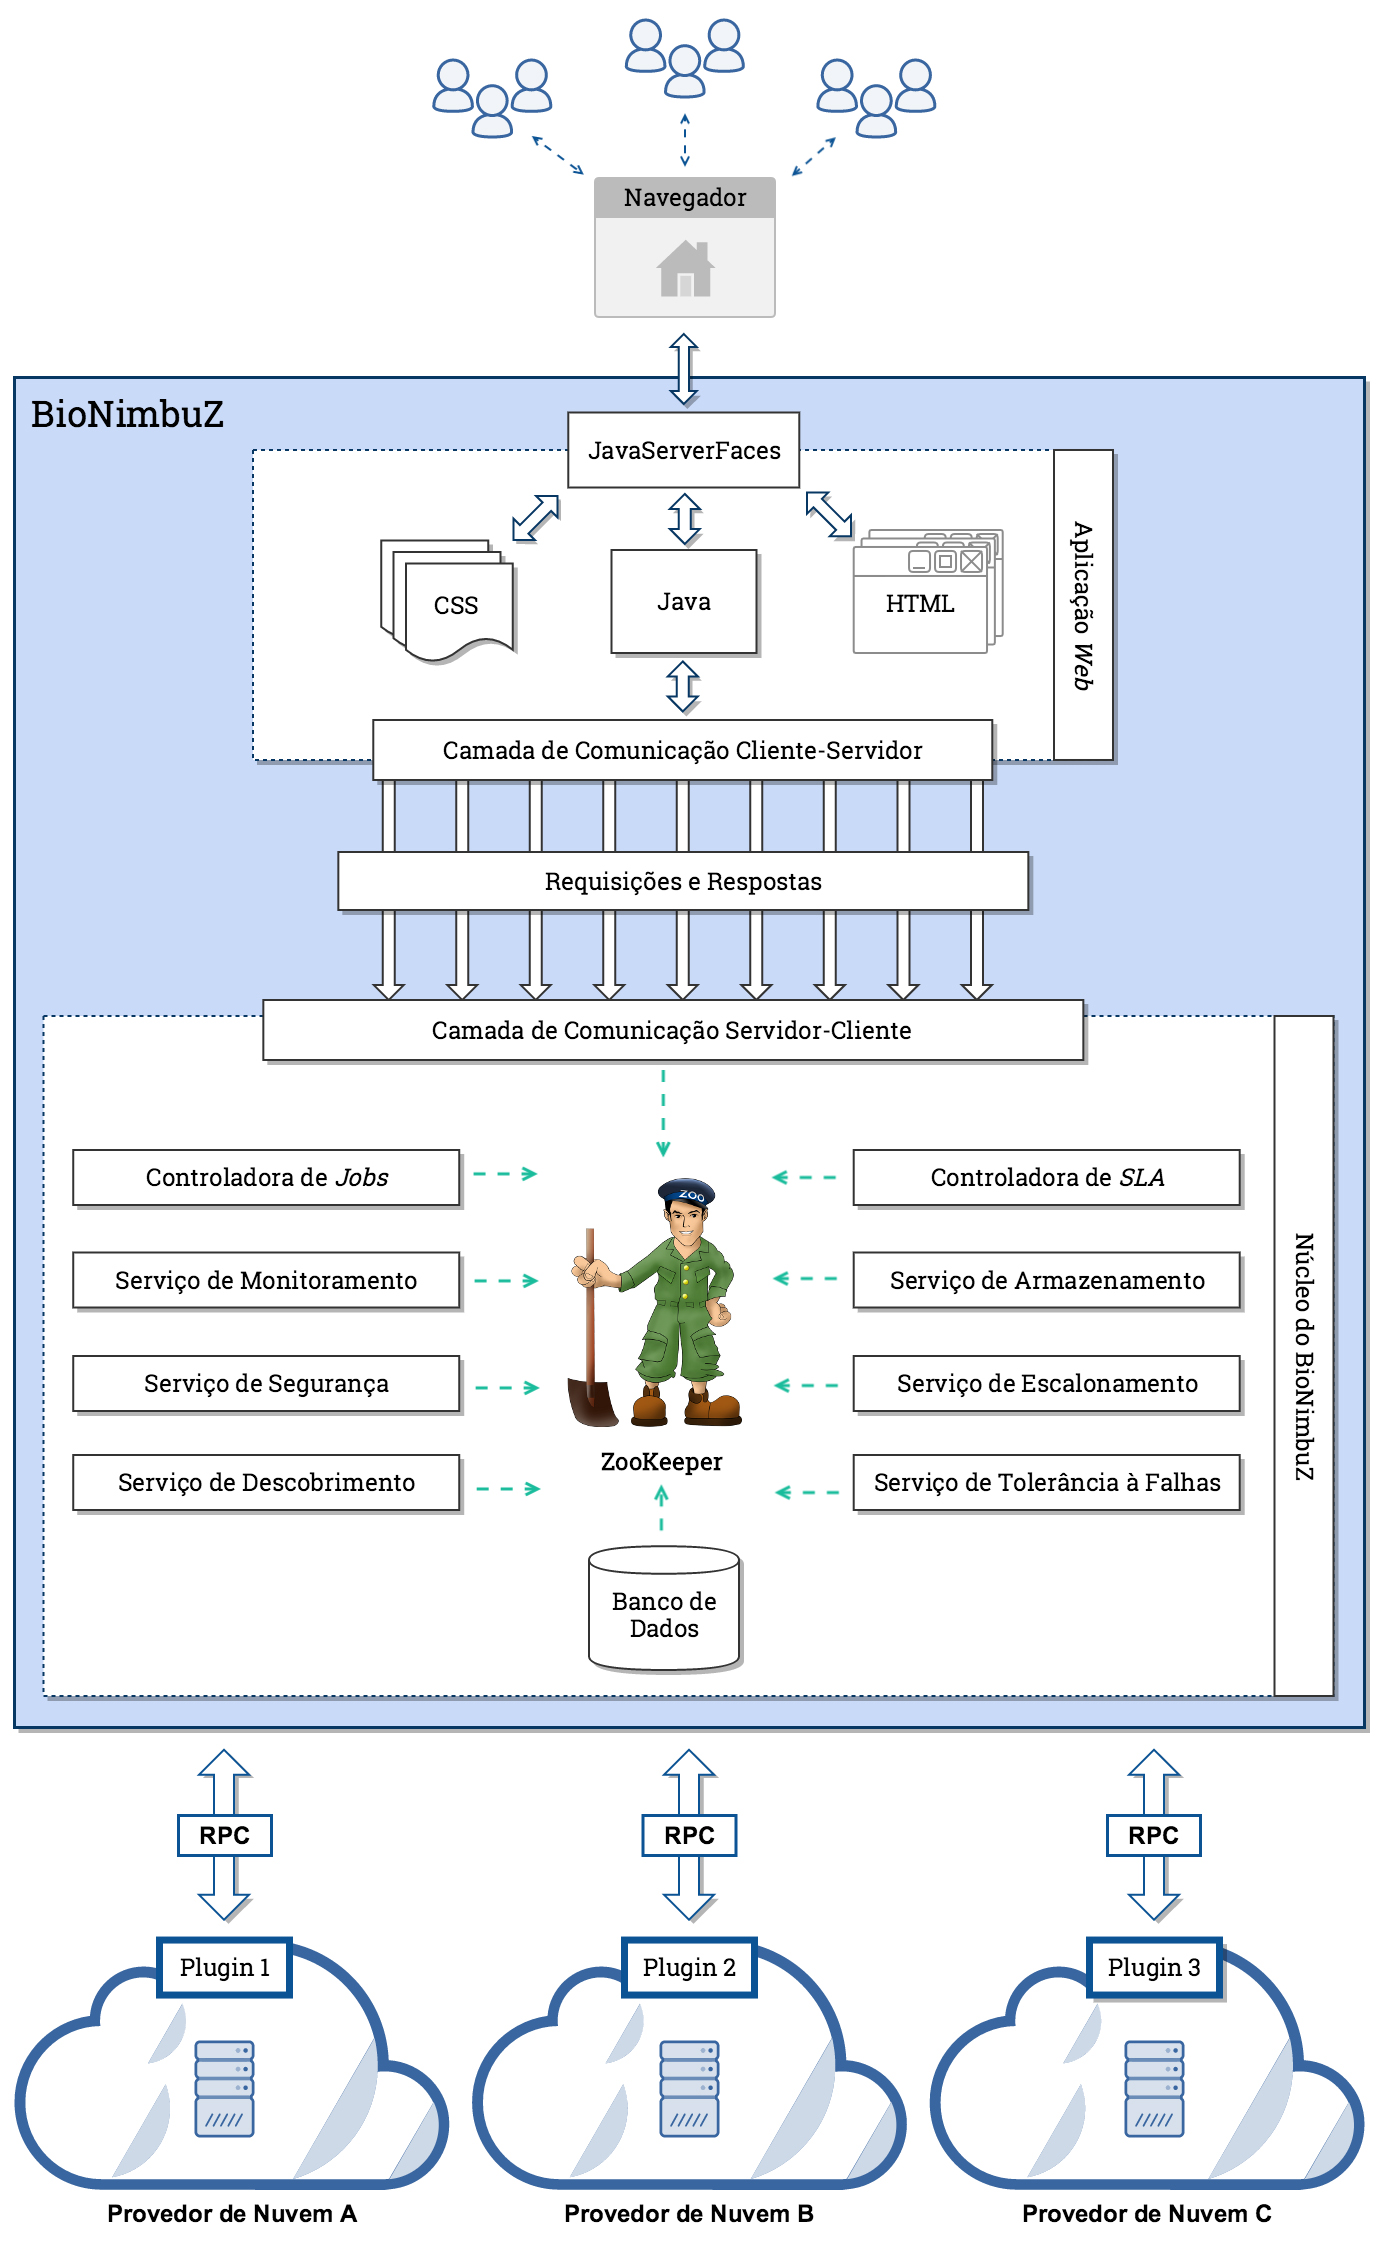
\includegraphics[scale=0.27 ]{nova_arquitetura.jpg}
	\caption{Nova Arquitetura do BioNimbuZ.}
	\label{fig:proposta_arquitetura}
\end{figure}

\begin{itemize}
	\item \textbf{Aplicação \textit{Web}:} Implementa o sistema gerenciador de \textit{workflows} científicos e utiliza a camada de comunicação para enviar requisições e receber respostas do núcleo.
    \item \textbf{Camada de Comunicação:} Implementa a troca de mensagens entre o núcleo e a aplicação \textit{web} utilizando \textit{webservices}, disparando requisições da aplicação \textit{web} para o núcleo e recebendo respostas do núcleo para a aplicação.
    \item \textbf{Núcleo:} Responsável pelo armazenamento de arquivos, escalonamento de \textit{jobs}, execução de \textit{workflows}, acesso ao banco de dados, descobrimento dos provedores e o gerenciamento de possíveis falhas.

\item \textbf{Infraestrutura:} Composta pelos provedores de serviço utilizados pelo BioNimbuZ e que compõem sua federação de nuvens.
\end{itemize}

A Seção \ref{cap5sec4} traz os detalhes de implementação da aplicação \textit{web} e a maneira a qual foi concebida.

\section{Aplicação \textit{Web}} \label{cap5sec4}
%	Para que o BioNimbuZ se tornasse acessível através da Internet, foi necessária a implementação de um método de acesso baseado em tecnologias Web. Para isso, foi desenvolvida um Sistema Gerenciador de \textit{Workflows} basado em interface gráfica utilizando a linguagem de programação Java, em conjunto com outros \textit{frameworks}, como: Java JSF, biblioteca de componentes visuais PrimeFaces, páginas HTML, códigos de estilo CSS.
    
	Este componente compreende o Sistema Gerenciador de \textit{Workflows} Científicos e deve prover meios para que usuários possam se logar no sistema BioNimbuZ através de uma interface gráfica acessível pela Internet e utilizem suas funcionalidades como envio de arquivos (que serão utilizados como entrada dos \textit{workflows} criados pelo usuário), exclusão de arquivos, visualização dos dados de saída gerados pela execução de seus \textit{workflows}, por exemplo. Pela interface, o usuário também deve ser capaz de criar e projetar seus \textit{workflows} de maneira gráfica, ligando passos, indicando dependências, incluindo argumentos e indicando quais arquivos de entrada serão utilizados.
    
Com os requisitos descritos na Seção anterior, foi projetada a implementação desse componente através da linguagem de programação Java e \textit{frameworks Web} (bibliotecas de \textit{software} que facilitam a implementação de funcionalidade relacionadas à sistemas voltados para \textit{internet}). 

Na implementação de uma aplicação \textit{Web}, o desenvolvimento é dividido em camadas e utiliza-se, normalmente, o padrão de projeto \textit{MVC} (\textit{Model-View-Controller}) \cite{design_patterns}. O padrão \textit{MVC} é utilizado no desenvolvimento de interfaces pela sua cartacterística de estar intimamente mapeado nos aspectos principais de uma interface: 

\begin{itemize}
	\item \textbf{Visualização:} Fornece a apresentação do dados presentes no Modelo.
    \item \textbf{Controlador:} Recebe os dados e comandos do usuário e determina o que isso significa para o Modelo.
    \item \textbf{Modelo:} Contém todos os dados e estados persistidos, geralmente em Bancos de Dados.
\end{itemize}

Dessa forma, o padrão \textit{MVC} contém exatamente esse três componentes: o \textbf{\textit{Model}} (Modelo), o \textbf{\textit{Controller}} (Controlador) e o \textbf{\textit{View}} (Visualização). A interação entre esses componentes pode ser descrita da seguinte maneira:

\begin{figure}[H]
	\centering
	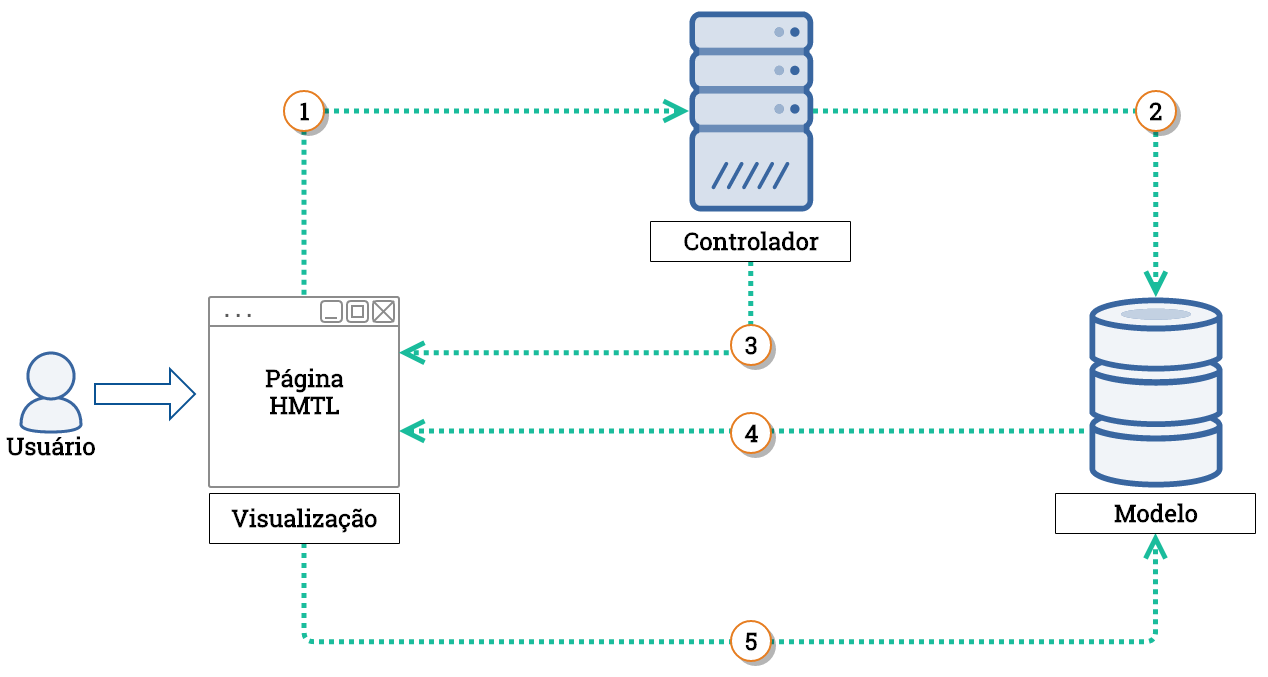
\includegraphics[scale=0.25 ]{padrao_mvc.png}
	\caption{Modelo \textit{Model-View-Controller}.}
	\label{fig:padrao_mvc}
\end{figure}

Na Figura \ref{fig:padrao_mvc}, o fluxo pode ser descrito como se segue:

\begin{itemize}
 	\item \textbf{(1):} O usuário realiza uma ação na página HTML.
    \item \textbf{(2):} O Controlador processa o comando e muda o estado de algum objeto no Modelo.
    \item \textbf{(3):} O Controlador envia um comando à Visualização para modificar os dados exibidos.
    \item \textbf{(4):} O Modelo notifica a Visualização de que os dados foram modificados.
    \item \textbf{(5):} A Visualização envia uma requisição ao Modelo pedindo o estado de algum dado.
\end{itemize}

Nesse contexto, diversos \textit{frameworks} surgiram voltados para o desenvolvimento de aplicações \textit{web}, tais como: \textit{Spring MVC} [41], \textit{Struts} [42], \textit{JSF} (\textit{JavaServerFaces}) [32], \textit{Play} [43], entre outros. Para esse projeto, o \textit{framework} escolhido foi o \textit{JSF}.

O \textit{JavaServerFaces} é uma especificação Java para a construção de interfaces de usuário baseadas em componentes para aplicações \textit{web}. Possui um modelo de programação dirigido a eventos, abstraindo os detalhes da manipulação e organização dos componentes, permitindo que o programador se concentre na lógica da aplicação.

Dessa forma, utilizando-se o padrão MVC descrito anteriormente, foi projetada e implementada a aplicação \textit{web} contendo os componentes necessários para o desenvolvimento do sistema gerenciador de \textit{workflows} científicos. 

\subsection{Camada de Modelo} \label{cap5sec4subsec1}

Geralmente a primeira fase do desenvolvimento de um software, é levantar os requisitos e definir as entidades principais do sistema, formando assim um modelo do sistema. As entidades de um sistema podem ser qualquer coisa que façam sentido na solução do problema específico, para o qual aquele sistema foi criado. Por exemplo, um usuário do mundo real pode ser mapeado em uma entidade de sistema chamada \textit{User} com uma lista de características, tais como: nome, Cadastro de Pessoa Física, Registro Geral, sexo, telefone, email, etc. A depender do sistema, aspectos específicos podem ser definidos. Por exemplo, em um sistema médico atributos como tipo sanguineo e densidade óssea são importantes, mas ao mesmo tempo, esses atributos, geralmente, não tem finalidade em um sistema bancário, por exemplo.

Assim, essa camada deve prover entidades mapeadas que façam sentido para o sistema (com atributos bem definidos) e também deve garantir que seu estado seja persistente e íntegro a cada inclusão, atualização ou deleção. 

Nesse cenário, foram mapeadas entidades importantes para o sistema BioNimbuZ e também foi desenvolvido o acesso a banco de dados para garantir a persistência dessas informações. O bando de dados escolhido foi o \textbf{MySQL} \cite{mysql_url} por ser confiável, de fácil instalação e manutenção e por possibilitar a replicação dos dados, evitando assim um ponto único de falhas. Foi definido que sua localização e seu método de acesso deveriam ser desenvolvidos no núcleo, conforme proposta de nova arquitetura apresentada na Seção \ref{cap5sec3}.

As principais entidades do sistema e seus respectivos atributos são descritos a seguir:

\begin{itemize}
	\item \textbf{\texttt{Usuário}:} Contém todos os dados necessários para identificar um usuário no sistema. A Tabela \ref{tab:atributos_usuario} apresenta todos os atributos de um Usuário.

		\begin{table}[H]
		\centering
		\resizebox{\textwidth}{!}{%
		\begin{tabular}{||c|c||}
			\hline
			\textbf{Atributo} & \textbf{Descrição}  \\
			\hline  
			\hline
			\multicolumn{1}{||l|}{\textbf{\texttt{id}}}				& \multicolumn{1}{l||}{Sequência de caracteres que identifica unicamente um usuário no sistema.} \\ 
			\hline
			\multicolumn{1}{||l|}{\textbf{\texttt{login}}}			& \multicolumn{1}{l||}{Contém o \textit{login} para o usuário entrar no sistema.} \\
			\hline
			\multicolumn{1}{||l|}{\textbf{\texttt{password}}}			& \multicolumn{1}{l||}{Senha utilizada para entrar no sistema.} \\  
			\hline
			\multicolumn{1}{||l|}{\textbf{\texttt{name}}}				& \multicolumn{1}{l||}{Contém o nome do usuário.} \\ 
			\hline
			\multicolumn{1}{||l|}{\textbf{\texttt{cpf}}} 				& \multicolumn{1}{l||}{Cadastro de Pessoa Física do usuário.}\\ 
			\hline
			\multicolumn{1}{||l|}{\textbf{\texttt{cellphone}}}		& \multicolumn{1}{l||}{Celular do usuário.}        \\ 
			\hline
			\multicolumn{1}{||l|}{\textbf{\texttt{storageUsage}}}		& \multicolumn{1}{l||}{Contém a soma de \textit{bytes} dos arquivos enviados pelo usuário ao sistema.}        \\
			\hline
			\multicolumn{1}{||l|}{\textbf{\texttt{List<FileInfo>}}}	& \multicolumn{1}{l||}{Contém a lista de arquivos pertencente ao usuário.}        \\
			\hline
			\multicolumn{1}{||l|}{\textbf{\texttt{List<Workflows}}}	& \multicolumn{1}{l||}{Lista de \textit{workflows} submetidos pelo usuário.}        \\
			\hline
		\end{tabular}
		}
		\caption{Lista de atributos da entidade \texttt{Usuário}.}
		\label{tab:atributos_usuario}
	\end{table}	
		
	\item \textbf{\texttt{FileInfo}:} Contém as informações acerca de arquivos que são enviados à plataforma BioNimbuZ e apresentado na Tabela \ref{tab:atributos_file_info}.
		\begin{table}[H]
		\centering
		\resizebox{\textwidth}{!}{%
		\begin{tabular}{||c|c||}
			\hline
			\textbf{Atributo} & \textbf{Descrição}  \\
			\hline  
			\hline
			\multicolumn{1}{||l|}{\textbf{\texttt{id}}}				& \multicolumn{1}{l||}{Identificador único do arquivo.} \\ 			
			\hline
			\multicolumn{1}{||l|}{\textbf{\texttt{name}}}				& \multicolumn{1}{l||}{Nome do arquivo.} \\ 			
			\hline
			\multicolumn{1}{||l|}{\textbf{\texttt{size}}}				& \multicolumn{1}{l||}{Tamanho em \textit{bytes} do arquivo.} \\ 			
			\hline
			\multicolumn{1}{||l|}{\textbf{\texttt{userId}}}			& \multicolumn{1}{l||}{Identificador do usuário que realizou o \textit{upload} deste arquivo.} \\ 			
			\hline
			\multicolumn{1}{||l|}{\textbf{\texttt{uploadTimestamp}}}	& \multicolumn{1}{l||}{Dia e horário do \textit{upload} do arquivo.} \\ 			
			\hline
			\multicolumn{1}{||l|}{\textbf{\texttt{hash}}}				& \multicolumn{1}{l||}{Contém o \textit{hash} do arquivo para verificação de sua integridade.} \\ 			
			\hline
			\multicolumn{1}{||l|}{\textbf{\texttt{payload}}}			& \multicolumn{1}{l||}{\textit{Bytes} contendo o arquivo em si.} \\ 			
			\hline
		\end{tabular}
		}
		\caption{Lista de atributos da entidade \texttt{}.}
		\label{tab:atributos_file_info}
	\end{table}	
	
	\item \textbf{\texttt{Job}:} Define um passo do \textit{workflow}. No BioNimbuZ, todo \textit{workflow} é composto por uma sequência de \textit{jobs}. Seus atributos são mostrados na Tabela \ref{tab:atributos_job}.

		\begin{table}[H]
		\centering
		\resizebox{\textwidth}{!}{%
		\begin{tabular}{||c|c||}
			\hline
			\textbf{Atributo} & \textbf{Descrição}  \\
			\hline  
			\hline
			\multicolumn{1}{||l|}{\textbf{\texttt{id}}}				& \multicolumn{1}{l||}{Identificado do \textit{job}.} \\ 			
			\hline
			\multicolumn{1}{||l|}{\textbf{\texttt{serviceId}}}		& \multicolumn{1}{l||}{Identificador do software computacional disponibilizado pelo BioNimbuZ.} \\ 			
			\hline
			\multicolumn{1}{||l|}{\textbf{\texttt{args}}}				& \multicolumn{1}{l||}{Campo opcional que contém os argumentos de entrada de um dado software.} \\ 			
			\hline
			\multicolumn{1}{||l|}{\textbf{\texttt{List<FileInfo>}}}	& \multicolumn{1}{l||}{Lista de arquivos de entrada daquele \textit{job}.} \\ 			
			\hline
			\multicolumn{1}{||l|}{\textbf{\texttt{output}}}			& \multicolumn{1}{l||}{Nome do arquivo de saída deste passo.} \\ 			
			\hline
			\multicolumn{1}{||l|}{\textbf{\texttt{dependencies}}}		& \multicolumn{1}{l||}{Contém os passos que devem ser executados antes da execução desse \textit{job}.} \\ 			
			\hline
		\end{tabular}
		}
		\caption{Lista de atributos da entidade \texttt{Job}.}
		\label{tab:atributos_job}
	\end{table}	
	
	\item \textbf{\texttt{Workflow}:} Descreve a entidade alvo desse sistema, o \textit{workflow} contendo sua lista de passos (\textit{jobs}). Seus atributos são mostrados na Tabela \ref{tab:atributos_workflow}.
		\begin{table}[H]
		\centering
		\resizebox{\textwidth}{!}{%
		\begin{tabular}{||c|c||}
			\hline
			\textbf{Atributo} & \textbf{Descrição}  \\
			\hline  
			\hline
			\multicolumn{1}{||l|}{\textbf{\texttt{id}}}			& \multicolumn{1}{l||}{Identificador do \textit{workflow}.} \\ 			
			\hline
			\multicolumn{1}{||l|}{\textbf{\texttt{List<Job>}}}	& \multicolumn{1}{l||}{Lista de \textit{jobs} que compõem o \textit{workflow}.} \\ 			
			\hline
			\multicolumn{1}{||l|}{\textbf{\texttt{datestamp}}}	& \multicolumn{1}{l||}{Dia e horário da criação do \textit{workflow}.} \\ 			
			\hline
			\multicolumn{1}{||l|}{\textbf{\texttt{userId}}}		& \multicolumn{1}{l||}{Identificador do usuário que criou o \textit{workflow}.} \\ 			
			\hline
			\multicolumn{1}{||l|}{\textbf{\texttt{description}}}	& \multicolumn{1}{l||}{Breve descrição do \textit{workflow}.} \\ 			
			\hline
			\multicolumn{1}{||l|}{\textbf{\texttt{status}}}		& \multicolumn{1}{l||}{Estado atual do \textit{workflow} (pendente, executando, pausado, com erros, etc).} \\
			\hline
		\end{tabular}
		}
		\caption{Lista de atributos da entidade \texttt{Workflow}.}
		\label{tab:atributos_workflow}
	\end{table}
\end{itemize}

Assim, com as entidades do sistema projetadas, passou-se ao desenvolvimento da próxima camada do modelo \textit{MVC}, a camada de visualização. Seus detalhes são apresentados na próxima Seção, \ref{cap5sec4subsec2}.

\subsection{Camada de Visualização} \label{cap5sec4subsec2}

Após o mapeamentos das entidades necessárias para o sistema gerenciador de \textit{workflow}, foi desenvolvida a camada de visualização do modelo \textit{MVC}. Para tal, foram implementadas páginas em \textbf{HTML} \cite{html_rfc} (\textit{Hypertext Markup Language}) utilizando componentes visuais da biblioteca \textit{Primefaces} \cite{primefaces_url}. O \textit{framework} \textbf{\textit{Primefaces}} possibilita utilizar componentes visuais ricos e de maneira simples, sem se preocupar em ajustar parâmetros visuais ou de programação. 

Isso significa que, utilizando o \textit{Primefaces}, não é necessário desenvolver os códigos de estilo \textit{CSS} \cite{css_rfc} (\textit{Cascading Style Sheets} - especificação que define como os elementos que compõem uma página, um documento ou aplicação \textit{web} serão exibidos). 

\textit{Primefaces} também possibilita a criação de páginas \textit{web} sem desenvolver código \textit{JavaScript} \cite{js_rfc} (linguagem de programação baseada em \textit{scripts}, utilizada na parte cliente de páginas \textit{web}, isto é, código executado no navegador do usuário), tornando o processo de desenvolvimento muito mais eficaz, dado que não é necessário desenvolver a interação entre os elementos. 

Essas duas características do \textit{Primefaces} facilitam a criação de páginas \textit{web}, possibilitando o desenvolvimento de páginas mais interativas e dinâmicas.

A partir da escolha de tecnologias, foram então desenvolvidas as páginas \textit{web} do sistema. O resultado será apresentado no \refCap{capitulo6}, o qual trata dos resultado obtidos com o desenvolvimento do sistema gerenciador de \textit{workflows}. A Tabela \ref{tab:tabela_clases_paginas} apresenta a lista de páginas e suas respectivas funções .

\begin{table}[H]
\centering
\resizebox{\textwidth}{!}{%
\begin{tabular}{||c|c||}
\hline
\textbf{Página \textit{HTML}} & \textbf{Função}  \\
\hline
\hline
\multicolumn{1}{||l|}{\textbf{\texttt{login.html}}}				& \multicolumn{1}{l||}{Página de \textit{login}} \\ 
\hline
\multicolumn{1}{||l|}{\textbf{\texttt{sign\_up.html}}}			& \multicolumn{1}{l||}{Página de cadastro de novos usuários} \\
\hline
\multicolumn{1}{||l|}{\textbf{\texttt{file\_upload.html}}}		& \multicolumn{1}{l||}{Página relativa à \textit{upload} de arquivos} \\  
\hline
\multicolumn{1}{||l|}{\textbf{\texttt{delete\_file.html}}}		& \multicolumn{1}{l||}{Página de deleção de arquivos do usuário} \\ 
\hline
\multicolumn{1}{||l|}{\textbf{\texttt{workflow\_composer.html}}} 	& \multicolumn{1}{l||}{Página de composição, \textit{design} e submissão de \textit{workflows}}\\ 
\hline
\multicolumn{1}{||l|}{\textbf{\texttt{workflow\_status.html}}}	& \multicolumn{1}{l||}{Página para visualização do \textit{status} dos \textit{workflows} gerenciados pelo usuário}        \\ 
\hline
\multicolumn{1}{||l|}{\textbf{\texttt{workflow\_history.html}}}	& \multicolumn{1}{l||}{Contém o histórico de execução de um determinado \textit{workflow}}        \\
\hline
\end{tabular}
}
\caption{Relação entre classes Java e páginas \textit{HTML}.}
\label{tab:tabela_clases_paginas}
\end{table}

A Seção \ref{cap5sec4subsec3} trata da Camada de Controle e as principais classes envolvidas em seu desenvolvimento.

\subsection{Camada de Controle} \label{cap5sec4subsec3}

Conforme o que foi exposto previamente, a camada de controle tem a responsabilidade de interpretar os dados enviados pelo usuário, a partir da camada de visualização (que neste projeto foi desenvolvida a partir de páginas \textit{HTML}), sinalizando ao sistema o que aqueles comandos representam. Essa passagem de dados, da página \textit{HTML} para as classes \textit{Java} é de responsabilidade do \textit{framework MVC JSF}.

Assim, foram desenvolvidas classes Java controladoras para tratar as requisições disparadas nas páginas \textit{web} de forma que houvesse uma correspondência entre as classes Java e suas respectiva páginas \textit{HTML}. Essa correspondência é mostrada na Tabela \ref{tab:tabela_java_paginas} e descrita a seguir:

\begin{table}[H]
\centering
\begin{tabular}{||c|c||}
\hline
\textbf{Classe Java} & \textbf{Página relacionada}  \\
\hline
\hline
\multicolumn{1}{||l|}{\textbf{\texttt{SessionBean}}}				& \multicolumn{1}{l||}{\texttt{login.html}} \\ 
\hline
\multicolumn{1}{||l|}{\textbf{\texttt{SignUpBean}}}				& \multicolumn{1}{l||}{\texttt{sign\_up.html}} \\
\hline
\multicolumn{1}{||l|}{\textbf{\texttt{FileUploadBean}}}			& \multicolumn{1}{l||}{\texttt{file\_upload.html}} \\  
\hline
\multicolumn{1}{||l|}{\textbf{\texttt{DeleteFileBean}}} 			& \multicolumn{1}{l||}{\texttt{delete\_file.html}} \\ 
\hline
\multicolumn{1}{||l|}{\textbf{\texttt{WorkflowComposerBean}}} 	& \multicolumn{1}{l||}{\texttt{workflow\_composer.html}}      \\ 
\hline
\multicolumn{1}{||l|}{\textbf{\texttt{WorkflowStatusBean}}}		& \multicolumn{1}{l||}{\texttt{workflow\_status.html}}        \\ 
\hline
\multicolumn{1}{||l|}{\textbf{\texttt{WorkflowHistoryBean}}}		& \multicolumn{1}{l||}{\texttt{workflow\_history.html}}        \\
\hline
\end{tabular}
\caption{Relação entre classes Java e páginas \textit{HTML}.}
\label{tab:tabela_java_paginas}
\end{table}

\begin{itemize}
	\item \textbf{\texttt{SessionBean}:} Esta classe tem como função principal realizar ações relacionadas à sessão do usuário no sistema, como por exemplo executar o \textit{login} e o \textit{logout}. Também deve manter as informações acerca do usuário (dados pessoais, lista de arquivos, lista de \textit{workflows} submetidos, etc) para consulta por outros componentes do sistema, funcionando, portanto, como um repositório de dados de usuários;
	\item \textbf{\texttt{SignUpBean}:} Controla o fluxo do sistema quando um usuário deseja se cadastrar na plataforma, isto é, verifica se o usuário já foi cadastrado previamente, e, em caso negativo, realiza sua inclusão, persistindo-o no banco de dados;
	\item \textbf{\texttt{FileUploadBean}:} Responsável por enviar os arquivos dos usuários à plataforma BioNimbuZ. Também realiza o tratamento do arquivo, verificando aspectos tais como: 
	\begin{enumerate}	
		\item \textbf{Extensão:} Verifica se a extensão do arquivo satisfaz àquela esperada pelo sistema;
		\item \textbf{Tamanho:} Certifica-se de que o tamanho do arquivo enviado não ultrapassa o limite estipulado;
		\item \textbf{Nome de Arquivo:} Verifica se aquele nome de arquivo já não foi previamente enviado ao sistema.
	\end{enumerate}		
	\item \textbf{\texttt{DeleteFileBean}:} Sua função é deletar um arquivo de usuário, enviando a requisição de exclusão para o núcleo do BioNimbuZ e mostrando o resultado ao usuário (arquivo excluído ou erro no processamento);
	\item \textbf{\texttt{WorkflowComposerBean}:} Essa classe é a principal classe do sistema gerenciador de \textit{workflows} desenvolvido. Ela controla a página relativa à composição dos \textit{workflows}, fazendo toda verificação e validação dos dados de entradas, dos parâmetro de execução, do \textit{design} do \textit{workflow}, etc;
	\item \textbf{\texttt{WorkflowStatusBean}:} Requisita ao núcleo do BioNimbuZ o estado de um determinado \textit{workflow}, enviando, para isso, seu \texttt{ID}. Formata os dados de retorno, enviando-os à página \textit{HTML} para serem mostrados ao usuário;
	\item \textbf{\texttt{WorkflowHistoryBean}:} Envia requisições ao BioNimbuZ pedindo o passo-a-passo da execução de um dado \textit{workflow} (\textbf{\textit{log}}). Com este \textit{log}, o usuário pode, por exemplo, rastrear possíveis erros, propor melhorias ao seu fluxo ou analisar o passo-a-passo de execução de seu \textit{workflow}. Por fim esta classe formata a resposta enviada pelo núcleo e a disponibiliza à página \textit{web}.
\end{itemize}

A listagem acima demonstra a maioria das classes Java desenvolvidas com objetivo de controlar a camada de visualização, mas não todas. Outras classes auxiliares também foram implementadas, mas, por possuírem menor importância, não foram aqui citadas.

Dessa forma, essas classes realizam a função de controle do modelo \textit{MVC} que norteia o desenvolvimento da aplicação \textit{web}. A próxima Seção, \ref{cap5sec4}, trata da solução desenvolvida à fim de tratar o problema de comunicação entre a aplicação \textit{web} e o núcleo do BioNimbuZ.

% \subsection{Casos de Usos} \label{cap5sec3subsec1}

% \subsection{Fluxos das Ações} \label{cap5sec3subsec2}

\section{Camada de Comunicação} \label{cap5sec5}

Um dos requisitos da solução proposta era que os componentes de software compostos pela aplicação \textit{web} e pelo núcleo do BioNimbuZ fossem desenvolvidos de maneira separada. Com isso, surgiu o problema de comunicação entre esses dois elementos.

Nesse contexto, a solução desenvolvida tem como base a comunicação utilizando-se \textit{webservices REST}(\textit{\textbf{RE}presentational \textbf{S}tate \textbf{T}ransfer}). \textit{REST} é definido como ``\textit{estilo de arquitetura para sistemas de hipermídia distribuídos, descrevendo os princípios de engenharia de software que guiam o e as restrições de interação escolhidos para manter esses princípios, enquanto contrastando-as com as restrições de outros estilos arquiteturais.}'' \cite{rest}. Voltado para sistema baseados na Internet, tem sido amplamente utilizado na integração de sistemas, pois utiliza operações definidas no protocolo \textit{HTTP} (tais como \textit{PUT}, \textit{GET} e \textit{DELETE}). Assim, softwares que ``entendam'' o protocolo \textit{HTTP}, podem utilizar, geralmente, soluções baseadas em \textit{REST}.

Dessa forma, para possibilitar a troca de mensagens entre a aplicação \textit{web} e o núcleo do BioNimbuZ, foi necessário o desenvolvimento de três entidades principais: \textbf{Requisições} (\textit{requests}), \textbf{Respostas} (\textit{responses}) e \textbf{Ações} (\textit{actions}). Estas foram implementadas como \texttt{interface} Java, à fim de manter o código o mais genérico possível. Suas responsabilidades são as que seguem:

\begin{itemize}
	\item \textbf{Ações:} Definem o comando à ser executado pelo núcleo, enviando-lhe uma requisição, à fim de se obter uma resposta com os dados requeridos;
	\item \textbf{Requisições:} De acordo com \cite{rest}, toda requisição feita à um servidor deve conter todo o conjunto de informações necessárias para sua completude, pois a comunicação não deve manter estado (\textit{stateless}). Assim, foram desenvolvidas requisições que contivéssem todos os dados necessários para a execução daquela Ação requisitada pela aplicação \textit{web};
	\item \textbf{Respostas:} Definem a mensagem devolvida pelo núcleo do BioNimbuZ para uma dada ação. É verificada o código \textit{HTTP} de resposta (\textit{status code}), esperando-se, geralmente, o código \texttt{HTTP 200}, que indica sucesso na requisição. Outros código são comuns, tais como o código \texttt{HTTP 500}, sinalizando erro interno do servidor e \texttt{HTTP 400}, que significa que uma requisição foi mal montada (\textit{Bad Request}).
\end{itemize} 

A partir dessas definições, foram desenvolvidas as implementações das \texttt{interfaces} \texttt{Action}, \texttt{ResponseInfo} e \texttt{RequestInfo}. A Tabela \ref{tab:classes_java_rest} apresenta entre as classes \texttt{Action} x \texttt{ResponseInfo} x \texttt{RequestInfo}.

\begin{table}[H]
\centering
\resizebox{\textwidth}{!}{%
\begin{tabular}{||c|c|c||}
\hline
\textbf{\textit{Action}} & \textbf{\textit{ResponseInfo}} & \textbf{\textit{RequestInfo}} \\
\hline
\hline
\multicolumn{1}{||l|}{\textbf{\texttt{DeleteFile}}} & \multicolumn{1}{l|}{\texttt{DeleteFileResponse}} & \multicolumn{1}{l|}{\texttt{DeleteFileRequest
}} \\
\hline
\multicolumn{1}{||l|}{\textbf{\texttt{GetWorkflowHistory}}} & \multicolumn{1}{l|}{\texttt{GetWorkflowHistoryResponse}} & \multicolumn{1}{l|}{\texttt{GetWorkflowHistoryRequest}} \\
\hline
\multicolumn{1}{||l|}{\textbf{\texttt{GetWorkflowStatus}}} & \multicolumn{1}{l|}{\texttt{GetWorkflowStatusResponse}} & \multicolumn{1}{l|}{\texttt{GetWorkflowStatusRequest}} \\ 
\hline
\multicolumn{1}{||l|}{\textbf{\texttt{Login}}} & \multicolumn{1}{l|}{\texttt{LoginResponse}} & \multicolumn{1}{l|}{\texttt{LoginRequest}} \\
\hline
\multicolumn{1}{||l|}{\textbf{\texttt{Logout}}} & \multicolumn{1}{l|}{\texttt{LogoutResponse}} & \multicolumn{1}{l|}{\texttt{LogoutRequest}} \\
\hline
\multicolumn{1}{||l|}{\textbf{\texttt{SignUp}}} & \multicolumn{1}{l|}{\texttt{SignUpResponse}} & \multicolumn{1}{l|}{\texttt{SignUpRequest}} \\
\hline
\multicolumn{1}{||l|}{\textbf{\texttt{StartWorkflow}}} & \multicolumn{1}{l|}{\texttt{StartWorkflowResponse}} & \multicolumn{1}{l|}{\texttt{StartWorkflowRequest}} \\
\hline
\multicolumn{1}{||l|}{\textbf{\texttt{Upload}}} & \multicolumn{1}{l|}{\texttt{UploadResponse}} & \multicolumn{1}{l|}{\texttt{UploadRequest}} \\
\hline
\end{tabular}
}
\caption{Relação entre classes Java e páginas \textit{HTML}.}
\label{tab:classes_java_rest}
\end{table}

\subsection{Implementação da Camada de Comunicação na Aplicação \textit{Web}} \label{cap5sec5subsec1}

Para permitir a execução de uma determinada \textit{Action}, e seus respectivos \textit{Requests} e \textit{Responses}, foram desenvolvidas duas classes Java para controlar seu fluxo, executando uma ação, enviando sua respectiva requisição e aguardando uma resposta. As responsabilidades dessas classes, chamadas \texttt{RestService} e \texttt{RestCommunicator}, estão listadas abaixo:

\begin{itemize}
	\item \textbf{\texttt{RestService}:} Contém a lista de métodos disponíveis na Camada de Comunicação. Outros componentes de software só podem requisitar um comando \textit{REST} a partir da instanciação desta classe e caso o respectivo método ter sido previamente implementado.
	\item \textbf{\texttt{RestCommunicator}:} É responsável por prover um passo a passo a ser seguido para realização da comunicação via \textit{REST} da classe \texttt{RestService}. Utilizando o padrão de projeto \textit{Strategy} \cite{head_first_book} em conjunto com o conceito de polimorfismo, executa os seguinte métodos definido na interface \textit{Action}:
	\begin{enumerate}
		\item \textbf{\texttt{ping()}:} Verifica o estado do núcleo do BioNimbuZ antes de toda requisição, efetuando o comando \textit{ping} \cite{ping_rfc}, podendo retornar verdadeiro (\texttt{\textit{true}}) ou falso (\texttt{\textit{falso}}). Em caso negativo, a requisição falha e retorna uma mensagem de erro ao usuário com a mensagem ``\textit{Erro Interno do Servidor}'', sinalizando a falha na comunicação com o núcleo;
		\item \textbf{\texttt{setup()}:} Realiza a configuração prévia do objeto à ser enviado ao núcleo do BioNimbuZ, suprindo necessidades da comunicação via \textit{REST}, tais como: instanciação do cliente \textit{REST}, \textit{set} das informações necessárias para a requisição, etc;
		\item \textbf{\texttt{prepareTarget()}:} Configura o endereço alvo (\textit{target}) daquela requisição. Aponta para uma \textit{URL} contendo o endereço IP do núcleo juntamente com o caminho do recuro \textit{REST} \cite{rest} que irá recepcionar a requisição setada;
		\item \textbf{\texttt{execute()}:} Executa a Ação desejada, realizando a operação \textit{REST} definida pela requisição (\textit{GET}, \textit{POST}, \textit{DELETE}, etc), retornando uma resposta para as classes de controle.
	\end{enumerate}
\end{itemize}

\subsection{Implementação da Camada de Comunicação no Núcleo do BioNimbuZ} \label{cap5sec5subsec2}

\section{Alterações realizadas no Núcleo do BioNimbuZ} \label{cap5sec6}   

À fim de se obter a integração da aplicação \textit{web} com o atual BioNimbuZ, diversas alterações foram realizadas no núcleo do sistema. Entre elas estão: 

\begin{itemize}
	\item Desenvolvimento da parte receptora das requisições enviadas pela aplicação \textit{web} (recursos \textit{REST} \cite{rest}). Para isso foi necessário desenvolver todas as entidades da aplicação \textit{web}, as quais foram descritas na Seção anterior, também no núcleo do BioNimbuZ;
	\item Desenvolvimento do método de acesso à base de dados \textit{MySQL}. Para isso foi utilizada a biblioteca de persistência \textit{Hibernate} \cite{hibernate_url};
	\item Formas de controle dos \textit{workflows} enviados à plataforma, gravando todo o caminho seguido para que, posteriormente, essa informação seja repassada para que o usuário possa rastrear e analisar sua execução. Para isso, foram realizadas melhorias na Controladora de \textit{Jobs} (\textit{JobController}), já que sua responsabilidade é o gerenciamento dos \textit{jobs}.
\end{itemize}

As

\subsection{Recursos \textit{REST}} \label{cap5sec6subsec1}
 

\subsection{Método de acesso à base de dados} \label{cap5sec6subsec2}


\subsection{Controle de \textit{Workflow}} \label{cap5sec6subsec3}

%Descrever a arquitetura do BioNimbuZ (Linha de comando, módulos, provedores, camadas...)
%-	Demonstrar o funcionamento anterior (linha de comando) e propor uma nova interface que dê %suporte ao desenvolvimento do novo módulo controlador de Jobs.
%-	Propor uma nova arquitetura baseada em aplicação WEB e comunicação com o núcleo via %webservices (Protocolo de troca de mensagens, tratamento de erros, ** solução de envio de %arquivos **).
%-	Propor uma nova política de upload de arquivos baseado em paralelização.
%-	Descrever as mudanças propostas (Protocolo de comunicação via REST, nova interface, %gerenciamento da execução de Jobs, nova política de envio de arquivos...)
%-	Explicar os temas: webservices, REST, servidor de aplicação, aplicação WEB, gerenciamento de %Jobs.
%-	Quais as vantagens e desvantagens das soluções propostas
%
%Descrever mudanças realizadas no BioNimbuZ
%-	Aplicação WEB
%-	Protocolo de Comunicação via WebServices
%-	Interface de Comunicação "Aplicação - Núcleo"
%-	Gerenciador de Estado dos Jobs (JobController)



